\documentclass[./JimHeneghanDissertation.tex]{subfiles}
\begin{document}
	\chapter{Methods}
		\section{Introduction}
			Electromagnetic simulations in this dissertation were performed using the Finite-Difference Time-Domain (FDTD) method. 
		\section{FDTD Overview}
			The Finite-Difference Time-Domain (FDTD) method is a technique for iteratively solving Maxwell's curl equations. Using the finite difference approximation, the equations are discreetized for computational use and thus is second order accurate. The modern method for FDTD simulation, initially proposed by Yee in 1966 REF, constructs a grid is constructed where the electric field components are offset in space by half a grid dimension as can be seen in <FIGURE>. We call a single cell of this arrangement the \textit{Yee Cell}. To calculate the electric field value at a grid point the simulation needs to know the value at that point one time step earlier and the magnetic field value in the surrounding grid points half a time step earlier. Thus, the simulation alternately calculates the entire magnetic field and in the simulation field before calculating the electric field one “half” time step later. 
			
			\begin{equation} \label{eq1}
			\begin{split}
				\nabla \times \mathbf{E} &= -\mu \frac{\partial \mathbf{H}}{\partial t} \\ 
				\frac{\partial \mathbf{H}}{\partial t} &= -\frac{1}{\mu} \nabla \times \mathbf{E} \\
				\frac{\mathbf{H}(t+\frac{\Delta t}{2}) - \mathbf{H}(t-\frac{\Delta t}{2})}{\Delta t} &= -\frac{1}{\mu} \nabla \times \mathbf{E}(t) \\
				\mathbf{H}(t+\frac{\Delta t}{2})  &= \mathbf{H}(t-\frac{\Delta t}{2}) -\frac{\Delta t}{\mu} \nabla \times \mathbf{E}(t) \\
			\end{split}
			\begin{split}
				\nabla \times \mathbf{H} &= -\varepsilon \frac{\partial \mathbf{E}}{\partial t} \\ 
				\frac{\partial \mathbf{E}}{\partial t} &= -\frac{1}{\varepsilon}\nabla \times \mathbf{H}\\
				\frac{\mathbf{E}(t+\Delta t)-\mathbf{E}(t)}{\Delta t} &= \frac{1}{\varepsilon}\nabla \times \mathbf{H}(t+\frac{\Delta t}{2}) \\
				\mathbf{E}(t+\Delta t) &= \mathbf{E}(t) + \frac{\Delta t}{\varepsilon}\nabla \times \mathbf{H}(t+\frac{\Delta t}{2}) \\
			\end{split}
			\end{equation}

			These equations are then solved for each vector component

			\begin{equation} \label{eq2}
			\begin{split}
				H_{x}(x,y,z)^{t+\frac{\Delta t}{2}}  &= H_{x}(x,y,z)^{t+\frac{\Delta t}{2}} -\frac{\Delta t}{\mu} (\frac{E_{y}^{t}(x,y+1,z) - E_{y}^{t}(x,y,z)}{\Delta y} - \frac{E_{z}^{t}(x,y,z+1) -E_{z}^{t}(x,y,z)}{\Delta z})\\
			\end{split}
			\end{equation}

			where $x, y, z$ represent coordinates in simulation space, $\Delta x, \ \Delta y, \ \Delta z$ are the lengths of the Yee cell in that dimension and $\Delta t$ is the simulation time step. As can be seen in \eqref{eq1} and \eqref{eq2} these formulations of Maxwell's curl equations are second order accurate. It has been shown that to mantain numerical stability the ratio of the time step to spatial step must satisfy the condition $c \Delta t \leq \frac{1}{\Delta x^{2} + \Delta y^{2} + \Delta z^{2}}$. The maximum value, $S_{c} = \frac{c \Delta t}{\Delta x^{2} + \Delta y^{2} + \Delta z^{2}}$, is known as the \textit{Courrant number} <REF>.

			\subsection{Generic explanation}
				The time domain nature of FDTD means that multiple frequencies of interest can be studied from a single simulation by using a broad band source. In this dissertation frequency domain analysis is performed with the FDTD code to produce electric field colormaps for a range of frequencies, reflectance and transmittance spectra and photonic band diagrams. 
			\subsection{Types of Analysis done with FDTD}
			\subsection{Utility of FDTD}
				The purpose of a FDTD simulation is to determine the electromagnetic response of some material structure. While simple methods for determining the response of layered structures, such as the transfer matrix method (TMM) <REF>, are effective, FDTD has the added flexibility to simulate more complexly patterned structures. The time domain nature of FDTD, unlike it's frequency domain counterparts, allows for broad band simulation while also allowing for the portrayal of specific frequency responses in post processing analysis. The method is accurate, robust and scalable. FDTD has been used to simulate macro scale objects, such as low visibility airicraft, scattering radar waves, cell phone signals interacting with human brain tissue and nano scale structures interacting with infrared scale wavelengths, which is the subject matter of this dissertation. Furthermore FDTD naturally handles nonlinear behavior, can handle anisotropic media and is easily parallelizable.

				\subsubsection{Limits of FDTD}

	\section{FDTD Adaptation}

			For all simulations performed a broadband, plane wave source was used. The time profile of the source was a Ricker wavelet \cite{Ricker:43} centered on $\lambda = 2.4\, \si{\um}$ ($4167\, \mathrm{cm}^{-1}$). This source injected a laterally uniform in time pulse using the total-field scattered-field (TFSF) interface \cite{Merewether:80}. The source was $y$-polarized and propagated in the negative $z$-direction. The use of the TFSF method enabled sensors to be placed above the TFSF boundary in order to record only the reflected field values.

			To prevent divergence in the simulation caused by edge reflections in the patterned Au layer, a convolutional perfectly matched layer (CPML) \cite{Gvozdic:17} boundary was used as the CPML has been shown to be more stable than a uniaxial perfectly matching layer (UPML) \cite{Sacks:95} absorbing boundary for simulations of this kind. Periodic boundary conditions were used in the transverse directions. In the positive and negative $z$-directions, the simulation was terminated by 50 perfectly matched layers. Due to the difference between the length scales of features in the transverse and longitudinal directions, the computational grid used cell sizes in the ratio of 10:10:1 in the $x$-, $y$- and $z$-dimensions, respectively. The resonance frequency of the patterned Au layer was found to be sensitive to the spatial resolution used in the simulation. Convergence testing was performed and a working resolution of $\mathrm{\Delta}x = 20 \, \si{\nm}, \ \mathrm{\Delta}y = 20 \, \si{\nm}, \ \mathrm{\Delta}z = 2 \, \si{\nm}$ was selected to be a good compromise between simulation accuracy and GPU memory limits.

			Reflectance and transmittance spectra were calculated by means of planar Poynting vector monitors which calculated frequency resolved components of the Poynting vector. The frequency resolved field components were calculated ``on the fly" using a discrete Fourier-transform (DFT) in the time domain. The Poynting vector was calculated from the field components using a plane wave expansion as detailed in Ref.~\cite{Rumpf:20}. The incident field data required to normalize the results were similarly calculated. The individual components of the spectrally resolved electric field in a given plane (\textit{e.g.,} at the vacuum/hBN interface) could be output for further analysis and visualization.  

			The various components of the device were modelled as follows. The hBN layer was simulated using a tensor Lorentz model, \textit{i.e.,}

			\begin{equation}
			  \bm{\varepsilon}_\mathrm{hBN}(\omega) = \begin{pmatrix} \varepsilon_{x}(\omega) & 0                       & 0                       \\
			    0                       & \varepsilon_{y}(\omega) & 0                       \\
			    0                       & 0                       & \varepsilon_{z}(\omega)\end{pmatrix},
			\end{equation}

			\noindent where
			\begin{equation}
			  \varepsilon_{k}(\omega) = \varepsilon_{k}(\infty) + \frac{S_{k} \omega_{k}^{2}}{\omega_{k}^{2} - i\gamma_{k}\omega - \omega^{2}},
			\end{equation}

			\noindent $\varepsilon_{k}(\infty)$ is the $k^{th}$ component (where $k=x,y,z$) of the dielectric function at infinity, $\omega_{k}$ is the frequency of a transverse optical phonon propagating in the $k^{th}$ direction, the factor $S_{k} \omega_{k}^{2}$ can be written in the form $\varepsilon_{k}(\infty)(\omega_\mathrm{LO}^2 - \omega_\mathrm{TO}^2) $  \cite{Kumar:15}, showing the explicit dependence on the longitudinal optical (LO) and transverse optical (TO) phonon frequencies. Given the polarization of the excitation source (see Fig.~\ref{fig:1}) the in-plane parameters used in this research were $\varepsilon_{x,y}(\infty) = 4.87$, $S_{x,y} = 0.61$, $\hbar\omega_{x,y} =  170.1 \, \si{\milli\eV}$. The out-of-plane parameters were  $\varepsilon_{z}(\infty)= 2.95$, $S_z = 0.61$,  $\gamma_z =  0.25\, \si{\milli\eV}$, and $\hbar \omega_{z} =  92.5 \, \si{\milli\eV}$ from Ref.~\cite{Jiang:18}. The notable exception was the planar damping constant $\gamma_{x,y}$, which has been shown to have a strong thickness dependence by Caldwell \textit{et al}. \cite{Caldwell:14}. Using results from the Caldwell group, as detailed in the supplemental materials section of that paper, the appropriate value of $\gamma_{x,y}$ for a film thickness of $80\, \si{\nm}$ was found to be $3.97\, \si{\milli\eV}$.

				\begin{figure}[!htb]
				  \centering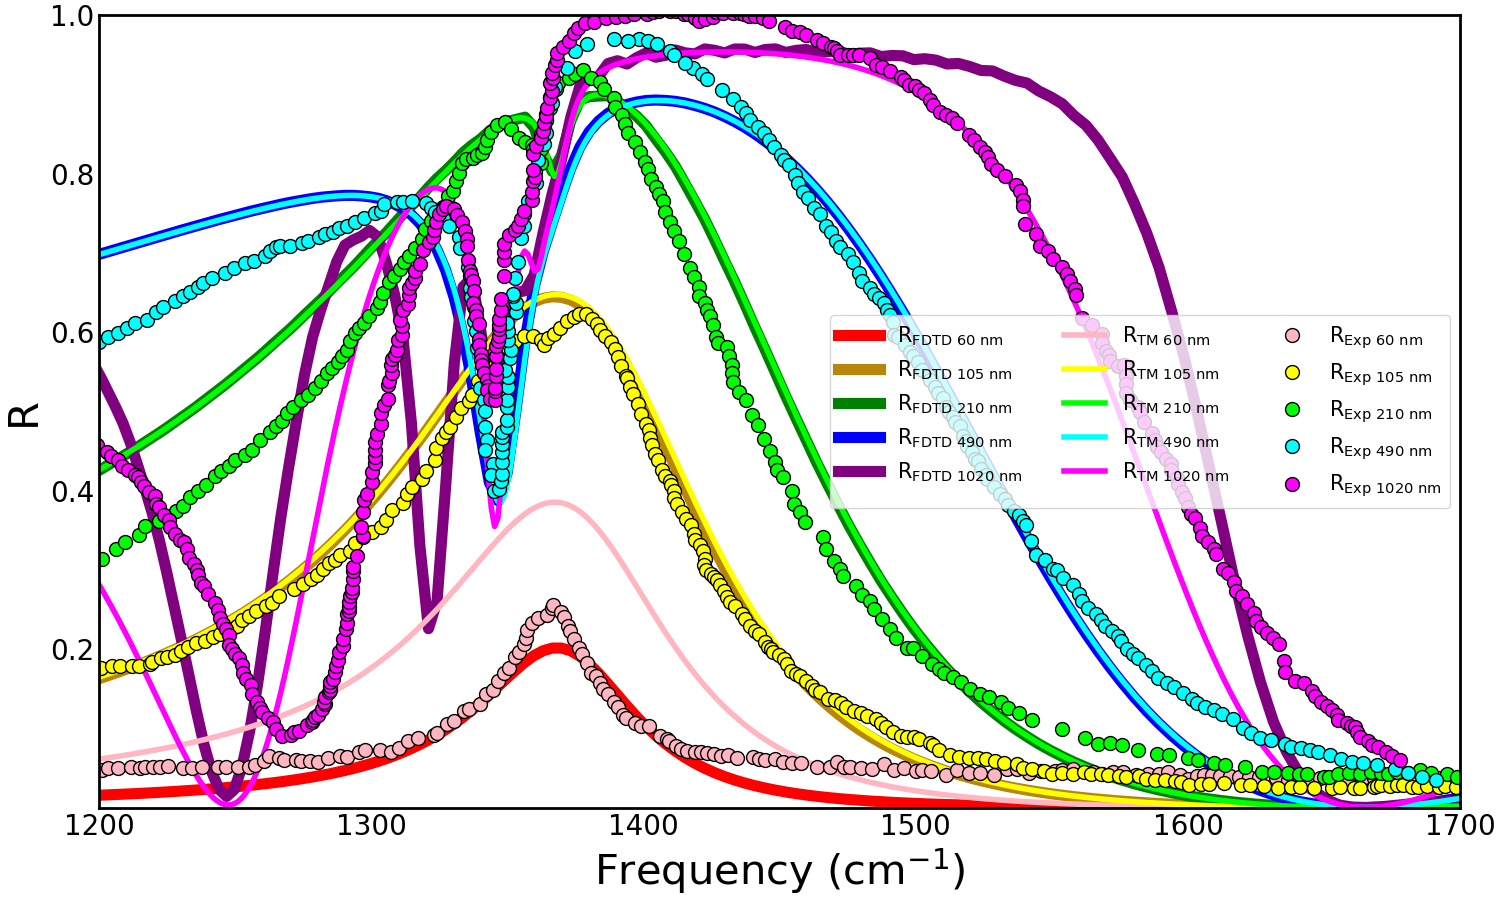
\includegraphics[width=0.45\textwidth]{Figures/CaldTMFDTD_hBN.png}
				  \caption{Reflectance spectra for various thicknesses of hBN. The dots are digitized data from Caldwell \textit{et al} \cite{Caldwell:14}, the dark solid lines are the spectra calculated using the transfer matric method, the light solid lines are spectra calculated from FDTD simulations. \textcolor{red}{note for Dr D. I intend to replace this figure with a 3 pane image. (a) will be the figure shown here but with one of the solid lines replaced with dashes and possibly one less thickness. Pane (b) will be the fitted curve that was used to calculate gamma. Pane (c) will be the FDTD and TMM RTA spectra. This section may be better placed in chapter 2}
				  }
				  \label{fig:2a}
				\end{figure}


		 	The Au film was simulated using wavelength dependent refractive index data as detailed by Ciesielski \textit{et al.}  \cite{Ciesielski:18} to fit to a Debye/Drude model, \textit{i.e.,}
			
			\begin{equation}
			  \varepsilon_\mathrm{Au}(\omega) = \varepsilon_\infty + \frac{\varepsilon_s - \varepsilon_\infty}{1+i\omega\tau_0} + \frac{\sigma}{i\omega\varepsilon_0},
			\end{equation}

			\noindent
			where $\varepsilon_\infty = 3.231$ is the dielectric function at infinity, $\varepsilon_\mathrm{s} = -1.598\times 10^4$ is the static dielectric constant, $\tau_0 =1.425\times 10^{-14}\,\si{\s}$ is the relaxation constant and $\sigma = 1.006\times 10^6\,\si{\siemens.m^{-1}}$ is the conductivity of Au, respectively. $\varepsilon_0$ is the permittivity of free space.
			Finally, the $\mathrm{SiO}_{2}$ substrate was simulated using a simple dielectric with $\varepsilon_\mathrm{SiO_2} = 2.127$. For implementation within the FDTD method, auxiliary differential equation (ADE) finite-difference approximations were derived from  the frequency dependent dielectric functions using the $Z$-transform method \cite{Sullivan:96,Sullivan:13}.


			In addition to the structure, denoted the ``coupled device" (CD), depicted in Fig.~\ref{fig:1}, several other auxiliary structures were simulated. In order to validate the models of the dispersive materials used in this work, thin films of Au and hBN in vacuo were simulated and the normal incidence absorptance, $A(\omega)$, spectrum for each of the films was calculated using $A(\omega) = 1 - [T(\omega) + R(\omega)]$, where $T(\omega)$ and $R(\omega)$ are the transmittance and reflectance spectra, respectively. These absorptance spectra were compared with the absorptance spectra calculated for the corresponding film using the transfer matrix (TM) method \cite{MacLeod:01} and excellent agreement between the two methods was observed.

			Several other structures were simulated for comparison with the coupled device (CD): (i) The ``bare device" (BD), this device is identical to the coupled device, but  with the hBN layer removed. This device does not support phonon-polaritons. (ii) The  ``uncoupled device I" (UDCI), this device is identical to the coupled device, but  with the hBN layer replaced with an equal thickness anisotropic layer that has $\varepsilon_{k}(\infty)$ equal to the values for hBN, but the resonant behavior removed by setting $S_{k} = 0$. This device does not support phonon-polaritons. (iii) The ``uncoupled device II" (UCDII), this device is identical to the coupled device, but with the nanopatterned Au layer replaced with an equal thickness layer of nanopatterned Si modelled by a frequency independent dielectric constant, $\varepsilon_\mathrm{Si} = 11.73$; this device does not support plasmons.

		
		\section{Sources}
			In order to perform useful stimulations an electromagnetic excitation needs to be introduced. Two common methods for this are discussed here: a pointwise hard source and a total field/scattered field (TFSF) source. For either source a time domain function is used to evolve the field value(s) at a specified location within the simulation space. While a harmonic source could be used this would fail to utilize the broadband frequency functionality of FDTD. For this reason much of the work in this dissertation was done using simulations excited by a Ricker wavelet <REF>. 
			\subsubsection{The Ricker Wavelet}

				\begin{equation} \label{rickereq}
					\nu_{r}(t)=(1-2(\pi \nu_{p}(t-d_{r})^{2}))e^{-(\pi \nu_{p}(t-d_{r})^{2})}
				\end{equation}




			Where $\nu_{p}$ is the peak frequency and $d_{r}$ is the temporal delay. The Ricker wavelet, \eqref{rickereq}, is a pulsed source equivalent to the second derivative of a Gaussian. The pulsing of the source enabled broad band simulations to be performed. Unlike a Gaussian pulse there is no dc component. The delay was able to be set such that the source "turned on" gradually. This gradual nature combined with a lack of a dc component reduced the occurrence of non-physical numerical artifacts in simulations. The spectral content was centered around a peak frequency in the spectral range of interest for each study. 

			\subsection{Point Sources}
				A point source in FDTD is simulated by varying a single (or array of single) grid points using a source function of the form discussed in the previous section. These sources are useful for simulating dipoles or artificial point sources, such as an afm tip. 

			\subsection{TFSF Source}
				A Total Field Scatter Field (TFSF) source allows the simulation of a "one-way" plane wave. By subtracting the backwards propagating portion of the source from the grid point half a cell dimension "behind" the source a space in the simulation is created where only non-negligible electric or magnetic field strength is due to signal which has been reflected, or scattered, from an object in the simulation. This is particularly useful when it comes to calculating reflection spectra.
				 
		\section{Boundary Conditions}
			In order to simulate realistic structures it was necessary to incorperate boundaries into our simulation. For periodic structures their properties were assertained by utilizing \textit{periodic} boundaries. Where a photonic band structure was the desired output these boundaries were varried to become Bloch periodic boundaries. In the case of a terminal boundary, such as an "infinite" substrate or incident medium, an absorbing boundry was used called a Perfectly Matched Layer (PML). 

			\subsection{PEC Boundary}

			\subsection{Periodic Boundary}
				To simulate an infinite sheet of meta materials the most basic unit cell was repeated `infinitly'. This was accomplished by bounding the simulation in the $x$- and $y$-direction with a periodic boundary. this is accomplished by updating the discreetized curl equation along the upper boundary (lower boundary for the magnetic field curl equation) explicitly. An example can be seen in \eqref{periodiceqn}
			\begin{equation} \label{periodiceqn}
				E_{y}^{t}(x,0,z) - E_{y}^{t}(x,N_{y},z)
			\end{equation}

				Where $N_{y}$ is the size of the simulation space in the $y$-direction. When the cells at $y=N_{y}$ are updated the term $E_{y}^{t}(x,y+1,z)$ is replaced with $E_{y}^{t}(x,0,z)$. Thus any signal exiting through a cell along the $y=N_{y}$ boundry reenters the simulation at $y=0$. To create an infinite two dimensional simulation space this procedure is repeated along the $x$ axis as well. 

				\subsubsection{Bloch Periodic Boundary}
			\subsection{Perfectly Matched Layers}
			
				\subsection{UPML}
				\subsection{CPML}

		\section{Materials Models}
			\subsection{Isotropy}
				\subsubsection{Isotropic}
				\subsubsection{Anisotropic}
				\subsubsection{Diagonally Anisotropic}
			\subsection{Dielectric Materials}
			\subsection{Dispersive materials}
				\subsubsection{Z Transform}
				\subsubsection{Drude Model}
				\subsubsection{Debye Drude Model}
				\subsubsection{Lorentz}
				\subsubsection{Diagonally Anisotropic}

		\section{Sensors}
			\subsection{Time domain sensors}
			\subsection{Frequency Domain Sensors}
				\subsubsection{Heat Maps}
				\subsubsection{RTA Spectra}

		\section{Analysis Tools}
			\subsection{Types}
				\subsubsection{Spectral}
				\subsubsection{Photonic Band}
				\subsubsection{Dispersion}
				\subsubsection{Heat Map}
			\subsection{Imaging}
			\subsection{Raster Dispersion}
		\section{Other Methods}
			\subsection{Transfer Matrix}



\end{document}